\documentclass[12pt]{article}
\date{}
\usepackage{tabularx}
\usepackage{capt-of}
\usepackage{caption}
\usepackage[most]{tcolorbox}
\usepackage[table]{xcolor}
\usepackage[backend=biber,
style=apa, sorting=nyt, defernumbers=true]{biblatex}
\addbibresource{referencias.bib}
\usepackage{setspace}
\setlength\bibitemsep{1.2\baselineskip}
\DeclareFieldFormat{labelnumber}{[#1]}
\definecolor{lavanda}{rgb}{0.827, 0.827, 1}
\definecolor{crema}{RGB}{251, 221, 173}
\usepackage{graphicx}
\usepackage{amsfonts}
\usepackage{amsmath}
\usepackage[colorlinks=true, linkcolor=blue, urlcolor=blue, citecolor=blue]{hyperref}
\usepackage[margin=2cm]{geometry}
\usepackage[spanish]{babel}
\usepackage{anyfontsize}
\usepackage{float}
\renewcommand\normalsize{\fontsize{14}{16}\selectfont}
\setlength{\parindent}{0pt}       

\begin{document}

\begin{titlepage}
    % Logo arriba izquierda
    \raggedright
    
\includegraphics[scale=0.1]{udec} % <<--- logo
    
    % Espacio
    \vspace{3cm}
    
    % Título centrado con líneas arriba y abajo
    \centering
    \rule{0.7\textwidth}{1pt} \\[0.5cm]
    {\Huge\bfseries \textsc{Laboratorio N°1} \par}
    \vspace{0.5cm}
    \rule{0.7\textwidth}{1pt}\par
    
    \vfill
    
    % Autores centrados
    {\Large \textsc{Maximiliano Concha \\ Ignacio Villagrán \\ Iván Barría} \par}
    \vspace{0.5cm}
    {\Large \textsc{Profesor/Ayudante: \\ Claudio Alonso Faúndez Araya \\ Nikola Alexander Fabián Salazar Varas}}    \\
    \vspace{1cm}
    {\large Universidad de Concepción \\ 22 de septiembre de 2025}
\end{titlepage}
\newpage
\section*{Introducción}
A lo largo de la historia de la termodinámica, el estudio de los gases y 
su comportamiento frente a distintas condiciones (como de presión, 
volumen y temperatura) constituye uno de los pilares fundamentales de 
esta rama de la física. Las leyes de los gases ideales nos dan las 
herramientas para comprender y poder predecir el comportamiento de los 
sistemas a estudiar -en particular sistemas gaseosos-.  En el presente 
laboratorio se busca comprobar mediante una simulación (disponible en la 
siguiente pagina web \url{https://phet.colorado.edu/sims/html/gas-properties/latest/gas-properties_es.html}) 
dichas leyes, que explican de manera muy precisa como se comportan los 
gases bajo ciertas condiciones iniciales. \\

Sirviéndonos de la simulación, se entregaran gráficos que evidencien las 
relaciones entre las propiedades termodinámicas anteriormente mencionadas.
De este modo, mediante los datos obtenidos, se tiene como expectativa 
observar la validez de las leyes vistas a lo largo del curso como las 
leyes de Boyle, Charles y Gay-Lussac, y como consecuencia observar la 
validez de la ecuación general de los gases ideales $PV=nRT$. El estudio 
y análisis realizado permitirá  acrecentar la comprensión de los 
principios teóricos de manera experimental (gracias a los datos obtenidos 
de la simulación) y visual (entregando gráficos), a su vez acrecentando 
también el entendimiento de los principios matemáticos que rigen a todos 
estos procesos termodinámicos.

\section*{Marco Teórico}
Un gas ideal es un gas cuyas moléculas se mueven de manera aleatoria, pero sin ejercer fuerzas de atracción entre ellas y las moléculas ocupan una parte despreciable del volumen. \parencite{condetema}. La mayoría de los gases a presión atmosférica y temperatura ambiente se suelen tratar como gases ideales. \\

Las leyes de los gases ideales son una herramienta muy importante a la 
hora de estudiar y analizar el comportamiento de gases sometidos a ciertas 
condiciones iniciales, esta ley nos permite predecir el comportamiento de un gas cuando varían las propiedades termodinámicas de presión, volumen y temperatura. Aunque, fuera del caso ideal ningún gas real es completamente ideal, pero esta ley es una muy buena aproximación en muchas condiciones. En general, con gases reales, es aplicable para presiones bajas y temperaturas altas. \\

\textbf{Ley de los gases ideales:} La presión $P$, la temperatura $T$, y el volumen 
$V$ de un gas ideal, están relacionados por una simple fórmula llamada 
la ley del gas ideal, cuya expresión matemática es:
\[
PV=nRT
\]
Donde $P$ es la presión del gas, $V$ es el volumen que ocupa, $T$ es su 
temperatura, $R$ es la constante del gas ideal, y $n$ es el número de moles
del gas. \parencite{khanleygasesideales}. 
R es también conocido como el numero de avogadro, que según la revista National Geografic, ``es la cantidad que nos dice cuántas partículas hay en un mol de cualquier sustancia, convirtiéndose así en una de las herramientas más importantes para comprender el mundo a nivel molecular''. \parencite{nationalgeographic_avogadro_2022} \\

Las siguientes leyes son casos particulares de la ley de los gases ideales,
donde se mantiene una variable constante. $T_1, V_1, P_1$ son las condiciones
iniciales y $T_2, V_2, P_2$ las condiciones finales de temperatura, 
volumen y presión respectivamente.\\
\\
\textbf{Ley de Boyle:} Establece que la presión de un gas en un recipiente 
cerrado es inversamente proporcional al volumen del recipiente, cuando la 
temperatura es constante. \parencite{educaplusleyboyle} Matemáticamente se 
expresa como:
\[
P_1V_1=P_2V_2
\]

\textbf{Ley de Charles:} Establece que, a presión 
constante, el volumen de un gas es directamente proporcional a su 
temperatura absoluta. \parencite{masamleycharles} Matemáticamente, esta 
relación se expresa de la siguiente manera:
\[
\dfrac{V_1}{T_1}=\dfrac{V_2}{T_2}
\]

\textbf{Ley de Gay-Lussac:} Cuando aumenta la temperatura de una muestra 
de gas en un recipiente rígido, también aumenta la presión del gas. El 
aumento de la energía cinética hace que las moléculas de gas golpeen las 
paredes del recipiente con mayor fuerza, lo que genera una mayor presión.
\parencite{libretextsgaylussac} Su expresión matemática es:
\[
\dfrac{P_1}{T_1}=\dfrac{P_2}{T_2}
\]
Como se ve, cada ley representa cuando cierta propiedad termodinámica se mantiene constante, por lo que resulta conveniente buscar una manera de representar como se realizan estas variaciones de las propiedades termodinámicas del sistemas, todo esto se ve gráficamente en el diagrama presión volumen.

\begin{figure}[H]
    \centering
    \includegraphics[width=0.4\textwidth]{99cedc42242c922c1e5642c68bba1c7d0f6ef01e.png}  
    \caption{Diagrama Presión-Volumen \parencite{khanacademy_pv_diagrams_2025}}
    \label{diagramaPV}  
\end{figure}
Como se ve en la figura [\ref{diagramaPV}] ,este diagrama es una representación gráfica que muestra la relación entre la presión y el volumen de cierto sistema. Este ayuda a identificar procesos termodinámicos como las isotermas (La temperatura se mantiene constante, en el gráfico se ve como una hipérbola), los procesos isobáricos (la presión se mantiene constante, en el diagrama se ve reflejado como una recta a lo largo del eje $P$) y los procesos isobáricos (el volumen se mantiene constante, se ve representado como una recta a lo largo del eje $V$). De forma análoga se puede hacer un diagrama Presión-Temperatura o Volumen-Temperatura.
\section*{Materiales}
\begin{itemize}
    \item Recipiente con gas
    \item Pistón
    \item Termómetro
    \item Barómetro
    \item Regularizador de temperatura
    \item Bomba de moléculas
\end{itemize}

\section*{Procedimientos}
\begin{enumerate}
    
\item Para la primera simulación se mantuvo la temperatura constante en 300$K$ para luego depositar 50 partículas pesadas en  el recipiente ($n=50$). A este recipiente se le fue variando el ancho a las siguientes cantidades: 15$nm$, 13$nm$, 11$nm$, 9$nm$, 7$nm$ y 5$nm$, para tomar datos de como varia la presión. Luego se repitió la simulación de la misma manera pero con temperaturas constantes de 300$K$ y 600$K$, luego analizamos como varia la presión cuando variamos el ancho del recipiente para distintas cantidades de partículas pesadas ($n=50$, $n=100$ y $n=150$ para cada caso).

\item Luego se realizaron  3  simulaciones donde  se depositaron 50, 150 y 250 partículas pesadas, en el orden dado en cada simulación, para así mantener una presión constante de 5.8 $atm$, 17.5 $atm$ y 29.2 $atm$ respectivamente en cada caso, para luego analizar como varia el ancho del recipiente cuando este se pone a las siguientes temperaturas: 150$K$, 225$K$, 375$K$ y 450$K$, para todas la simulaciones.
\end{enumerate}
\section*{Resultados y Análisis}

La tabla y los respectivos gráficos de la simulación número 2, 3 y 4 son los siguientes:
\begin{figure}[ht!]
    \centering
    % Crear una minipágina para la tabla y la imagen
    \begin{minipage}{0.48\textwidth}
        % Tabla para el primer subplot (n=50)
        \centering
        \begin{tabular}{|c|c|}
            \hline
            \textbf{Temperatura (K)} & \textbf{Volumen (nm)} \\
            \hline
            150 & 5 \\
            225 & 7.5 \\
            375 & 12.5 \\
            450 & 15 \\
            \hline
        \end{tabular}
        \caption{Tabla de variaciones del ancho del recipiente para $n = 50$, $n= 150$ y $n=250$}
        \label{tabla3en1}
    \end{minipage} \hspace{0.04\textwidth}  % Espacio entre la tabla y la imagen
    
    \begin{minipage}{0.7\textwidth}
        % Imagen del gráfico (sustituir el nombre de archivo por el nombre de tu imagen)
        \centering
        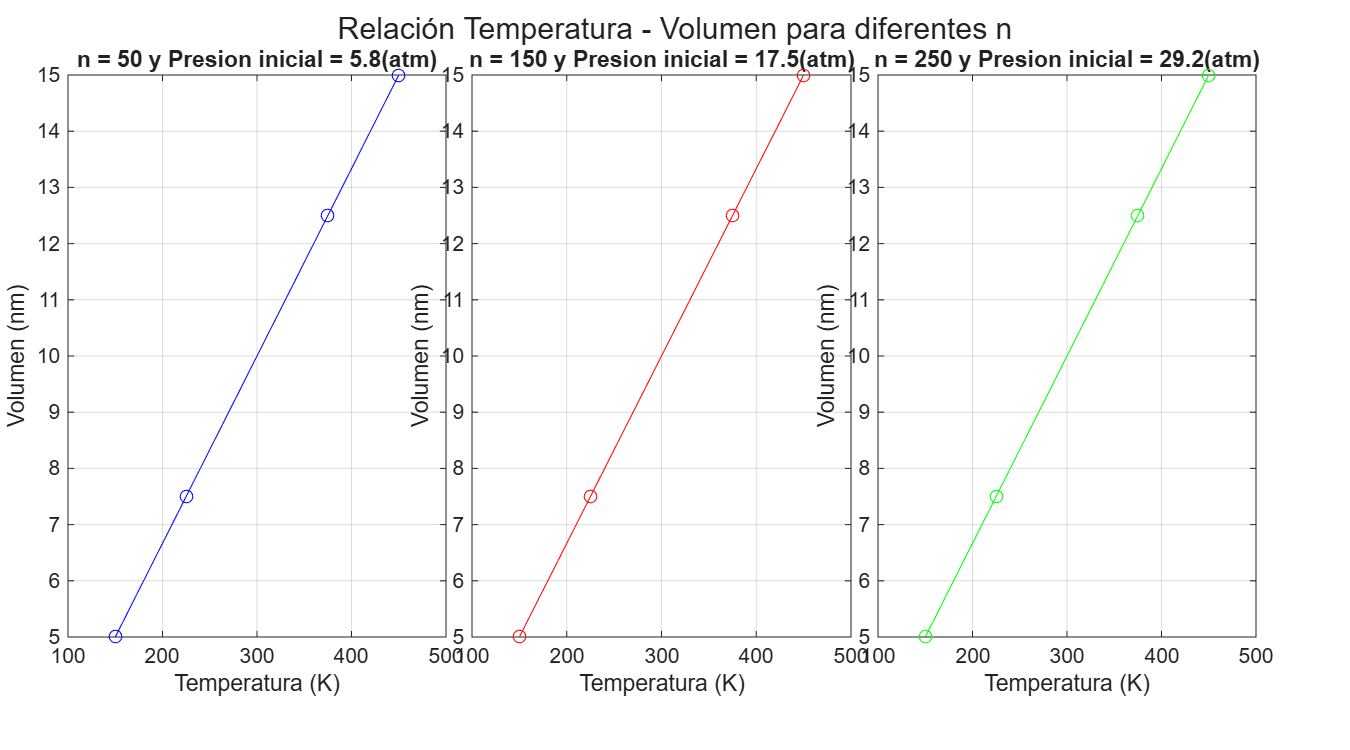
\includegraphics[width=\textwidth]{informe 2 termos/graficosTV.png}
        \caption{Gráfico de la relación Temperatura - Volumen para $n = 50$, $n= 150$ y $n=250$}
        \label{3grafico}
    \end{minipage}
\end{figure}
\\
Como se puede apreciar en la figura [\ref{3grafico}], en las diferentes simulaciones con distintas cantidades de partículas depositadas,  la longitud de nuestro recipiente varia hacia el mismo valor (con los valores de las temperaturas correspondientes), independiente de cuantas partículas tenga el recipiente y a cuanto se mantenga la presión constante debido a las partículas depositadas. Por esa razón tanto los gráficos como las tablas tienen los mismos valores, por lo que ocupamos solamente una tabla, como se ve en la figura [\ref{tabla3en1}] pero mantuvimos gráficos diferentes de las 3 distintas simulaciones. Para los 3 casos se observa que existe una relación lineal creciente entra la temperatura y el volumen, esto se ve relacionado directamente con la Ley de Charles y Gay-Lussac, ya que si la presión del gas se mantiene constante, al aumentar la temperatura del recipiente el volumen aumenta proporcionalmente. Aunque se esperaría que al varias $n$ o la presión inicial deberían cambiar las relaciones entre el volumen y temperatura en cada uno de los casos, pero no es así, ya que, como se ve en los tres gráficos de la figura [\ref{3grafico}], aunque los valores de $n$ y la presión inicial cambian, la relación Temperatura-Volumen sigue siendo lineal, confirmando el comportamiento de un gas ideal según la ecuación de estado de este mismo.  Como se mantiene $P$ constante se tiene en la ecuación de estado que el volumen es: 
\[V=\frac{nR}{P}T\]
Donde $\frac{nR}{P}$ es la pendiente de la recta. Por lo que, a medida que aumenta $n$, también lo hará la presión inicial, debido a eso todos los gráficos se mantienen igual, ya que sus pendientes son iguales para todos los casos.



Ahora con todos los datos ya tomados podemos empezar a responder la preguntas planteadas

\section*{Conclusión}


\newpage
\printbibliography[heading=bibintoc]

\end{document}